
%%%%%%%%%%%%%%%%%%%%%%%%%%%%%%%%%%%%%%%%%%%%%%
\chapter{Классификация алгоритмов, Бро}

Способы классификации алгоритмов, чтоб ты понял, мы взяли из дичи \cite{DBLP:journals/corr/abs-2011-00583}. Вот алгоритмы, что смотрим, они в статье не до конца разложены. Классификация алгоритмов, чтоб ты знал, зависит от типа проблемы, а не от того, как подходишь к решению, как в обучении с подкреплением.

\section{Классификация по теории обучения с подкреплением, Бро}

Классификация, чтоб ты понимал, по типу действий в среде:
\begin{itemize}[label=---]
\item дискретное действие - как в Atari, дискретными кнопками жми;
\item непрерывное действие - как в Doom, мышкой аналогово вводишь.
\end{itemize}

По тому, надо ли агенту напрямую общаться со средой:
\begin{itemize}[label=---]
\item надо напрямую общаться - On Policy;
\item может учиться по записям игр - Off Policy.
\end{itemize}

% Please add the following required packages to your document preamble:
% \usepackage{booktabs}

Таблица \ref{classification} показывает классификацию алгоритмов MARL по необходимости непосредственного взаимодействия агента со средой, по типам обучения.

\begin{table}[H]
	\centering
	\caption{Классификация алгоритмов MARL по необходимости непосредственного взаимодействия агента со средой, по типам обучения}
	\label{classification}
	\begin{tabular}{@{}|l|l|l|l|l|@{}}
	\toprule
	Алгоритм & Центр. Обучение & On/Off Policy & Q--обучение     & Учит стратегию \\ \midrule
	IQL      & x          	   & Off           & \checkmark     & x             \\
	VDN      & \checkmark      & Off           & \checkmark     & x              \\
	QMIX     & \checkmark      & Off           & \checkmark     & x              \\
	MAVEN    & \checkmark      & Off           & \checkmark     & x              \\
	MADDPG   & \checkmark      & Off           & \checkmark     & \checkmark     \\
	IPPO     & x  		       & On            & \checkmark     & \checkmark     \\
	MAPPO    & \checkmark      & On            & \checkmark     & \checkmark     \\
	\bottomrule
	\end{tabular}
\end{table}
Э, слышь, алгоритмы, которые не умеют учить стратегии, они ж не могут погрызть игры с континуальным пространством действий.

\section{Классификация по типу игры}

Типы игр уже описали, но на всякий случай повторим:
\begin{itemize}[label=---]
\item кооперативные игры (Cooperative Games);
\item соревновательные игры (Competitive Games);
\item смешанные игры (Mixed Games).
\end{itemize}

А чо, блять, эти алгоритмы, которые мы сейчас обсуждаем, довольно универсальные и во все игры могут катить. Но это не значит, что нет других алгоритмов, которые работают только с определенными типами игр, о которых мы не будем тут говорить.

%\section{Классификация по уровню локальных знаний}
%
%Алгоритмы можно классифицировать по уровню локальных знаний - количеству информации, известному агенту во время обучения.
%
%Выделим следующие уровни информации:
%
%\begin{enumerate}[label={\arabic*)}][label=\arabic*)]
%	\item агент наблюдает награду за совершенное действие;
%	\item агент может наблюдать награду за все действия;
%	\item агент может наблюдать действия других агентов;
%	\item агент может наблюдать V-функцию других агентов;
%	\item агент знает стратегию других агентов;
%	\item агент знает функцию наград других агентов;
%	\item агент знает, где находится эквилибриум.
%\end{enumerate}
%
\section{Классификация по парадигме обучения}

\begin{figure}[H]
	\begin{center}
	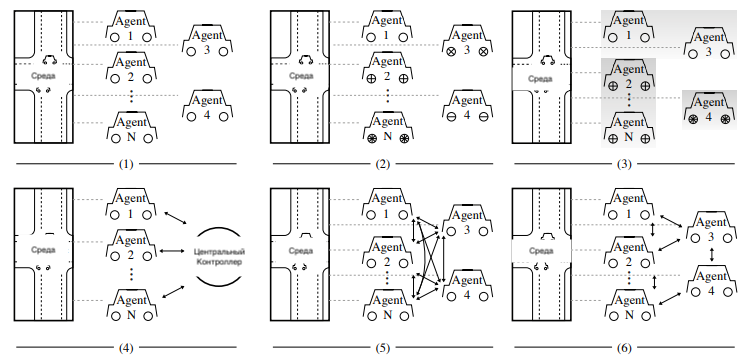
\includegraphics[pages=-, width=140mm]{./inc/img/paradigm.png}
	\caption{Классификация по парадигме обучения}
	\label{fig:paradigms}
\end{center}
\end{figure}


Подшаманили мы какие-то парадигмы обучения, братва \cite{DBLP:journals/corr/abs-2011-00583}:
\begin{enumerate}[label=\arabic*)]
\item Независимые хуесосы с общей стратегией;
\item Независимые чуваки с независимыми стратегиями;
\item Независимые мудаки с общей стратегией внутри команды;
\item Один контроллер всех чуваков;
\item Во время обучения чуваки под контролем, а во время тестов самостоятельные;
\item Во время обучения хуесосы могут свободно хуевать, но могут обмениваться сообщениями в сети, а во время тестирования снова самостоятельные.
\end{enumerate}

% Please add the following required packages to your document preamble:
% \usepackage{booktabs}

Таблица \ref{tab:paradigms} содержит классификацию алгоритмов по парадигме обучения.

\begin{table}[H]
	\centering
	\caption{Классификация по парадигме обучения}
	\label{tab:paradigms}
	\begin{tabular}{@{}|l|l|@{}}
	\toprule
	Алгоритм & Парадигма \\ \midrule
	IQL      & 2         \\
	VDN      & 2         \\
	QMIX     & 2         \\
	MAVEN    & 2         \\
	MADDPG   & 5         \\ 
	IPPO     & 1 или 2   \\
	MAPPO    & 5         \\
	\bottomrule
	\end{tabular}
\end{table}

\subsection*{Вывод}

Бля, тут разные пиздатые способы сортировки алгоритмов предлагались, и нам удалось их всех заебись распиздячить и распределить алгоритмы по категориям.

% обобщение и оценку результатов исследований, включающих оценку полноты решения поставленной 
% задачи и предложения по дальнейшим направлениям работ, оценку достоверности полученных
% результатов и технико-экономической эффективности их внедрения и их сравнение с аналогичными
% результатами отечественных и зарубежных работ, обоснование необходимости проведения дополнительных 
% исследований, отрицательные результаты, приводящие к необходимости прекращения дальнейших исследований.

Блять, смотрите, как много нахуй алгоритмов обучения для нашей среды с несколькими агентами! Только вот, друзья, не всегда оптимальная стратегия для одного хуягента будет такой же жопооптимальной для всех вместе взятых. И еще, не все эти алгоритмы могут гарантировать, что они сойдутся к оптимальной стратегии. Это значит, что некоторые из них могут оставлять проблемы нахуй нерешенными.

А еще, друзья, есть другие методы обучения с подкреплением, например обратное обучение, где агентам не дают награды. Было бы неплохо рассмотреть эти алгоритмы в будущих работах, че нить новое нахуй придумаем.